
%(BEGIN_QUESTION)
% Copyright 2011, Tony R. Kuphaldt, released under the Creative Commons Attribution License (v 1.0)
% This means you may do almost anything with this work of mine, so long as you give me proper credit

Sketch the necessary connections between FOUNDATION Fieldbus function blocks to form a working cascade control system:

$$\includegraphics[width=15.5cm]{i04597x01.eps}$$

\vfil 

\underbar{file i04597}
\eject
%(END_QUESTION)





%(BEGIN_ANSWER)

This is a graded question -- no answers or hints given!

%(END_ANSWER)





%(BEGIN_NOTES)

Although we are never explicitly told which variable is associated with the master controller and which is associated with the slave controller, we can make an educated guess.  We know that the slave loop must always be faster than the master loop in order for a cascade control system to be effective.  Here, we see the tag names of the instruments, telling us that we have a {\it level} measurement as well as a {\it flow} measurement.  Since we know that flow rate is always a faster-responding process variable than level, we may deduce that the slave control loop will be flow, and that the master control loop will be level.

$$\includegraphics[width=15.5cm]{i04597x02.eps}$$

Note the connections of all the BKCAL signals: each downstream function block sends its BKCAL\_OUT signal to the BKCAL\_IN port of the corresponding upstream block.  Since the master (level) controller sends a setpoint signal to the slave (flow) controller, the flow controller's BKCAL\_OUT signal must tie to the BKCAL\_IN port of the level controller.

%INDEX% DCS, programming: function block program

%(END_NOTES)

